\chapter{Le phénomène de percolation au c\oe{}ur des performances}
\label{sec:chap_percolation}

Nous avons montré au chapitre précédent que les $K$-polyèdres donnent exactement, niveau par niveau, les amas discrets de forte densité du modèle de \textsc{Hartigan} lorsque la densité est estimée par les $K$ plus proches voisins (\Def~\ref{def:HDC_discret} et \Th~\ref{th:cech_kpolyedres_knn}). 

La question se pose alors : cela apporte-t-il quelque chose aux performances théoriques de l'algorithme ?
La réponse est oui ! et le mécanisme à l'œuvre est la \emph{percolation}. 

C'est dans ce chapitre que tout l'intérêt de ce que nous avons appelé l'\emph{analyse persistante} apparaît : faire varier un rayon $r$ pour observer des composantes apparaître, croître puis disparaître en fusionnant, cela revient à observer un phénomène de percolation. Certaines statistiques sur cette composante géante permettent de quantifier ce que l'on peut espérer récupérer d'un amas de forte densité.

L'algorithme de Single-Linkage n'est pas consistant en dimension $p \ge 2$ à cause de ce phénomène de percolation ; il l'est seulement dans le cas très particulier de la dimension $p=1$, où ce phénomène de seuil n'a pas lieu. En dimension $p \ge 2$, on ne peut plus espérer retrouver intégralement tous les points de deux amas disjoints de forte densité, seulement une \emph{fraction}. L'importance (asymptotique) de cette fraction se lit dans la fonction de probabilité de percolation
\[
    \lambda\longmapsto \Theta^{\mathrm{fam}}_{K,p,r}(\lambda).
\]

%Le fil de ce chapitre est donc le suivant. 
En partant de la densité de génération $f$, l'on peut savoir à quoi va ressembler la hiérarchie asymptotique \emph{via} la probabilité de percolation. Dans le cas où $f$ est constante par morceaux et où deux amas denses sont séparés par un fond moins dense, cette lecture devient très simple grâce à un indice que nous avons baptisé la \emph{vitesse de percolation}.
Cette vitesse de percolation dépend de l'algorithme de clustering hiérarchique utilisé ; nous estimons donc cette vitesse en petite dimension pour comparer les $K$-polyèdres, le $K$-Robust Single-Linkage et $K$-DBSCAN.
Avantage certain à nos $K$-polyèdres !
Enfin, lorsque $K\to+\infty$, les niveaux de forte densité $K$-NN convergent asymptotiquement vers des excursions gaussiennes
\[
    E_a=\{x\in\mathbb R^p\mid G_p(x)\ge -a\}
\]
où $G_p$ est un champ gaussien stationnaire et $a$ mesure la fluctuation autour de la moyenne pour une intensité normalisée
\[
    \mu = K+a\sqrt K.
\]
Là encore, l'avantage des polyèdres est quantifiable.


\Contributions{Ce chapitre reprend \cite{BibiIstambul} et le généralise au cadre continu. Nous définissons la probabilité de percolation associée aux $K$-polyèdres, au $K$-Robust Single-Linkage et à DBSCAN ; nous montrons comment cette fonction contrôle la fraction asymptotiquement récupérable dans le modèle de \textsc{Hartigan} ; nous introduisons une vitesse de percolation que nous mesurons effectivement en petite dimension pour quelques valeurs de $K$ ; enfin, nous calculons le développement asymptotique de cette vitesse lorsque $K\to+\infty$. 
Les résultats concordent : les polyèdres percolent plus vite dans les amas denses, et sont donc \emph{fractionnellement} plus consistants.}

\Remarque{Il nous a paru plus pertinent de tout définir dans ce chapitre par rapport à l'intensité $\lambda$ ; nous fixons donc dès maintenant le rayon $r$ tout au long de ce chapitre à
\[
    r=\frac12.
\]}


\section{Introduction à la percolation}

Le terme latin \emph{percōlātĭō} signifie une « filtration » (\textsc{Gaffiot}). De l'eau \emph{percole} à travers une roche lorsqu'elle s'y infiltre et la traverse par un réseau géant formé de petits pores. Le modèle mathématique de la percolation fut introduit par \textsc{Broadbent \& Hammersley} \cite{BroadbentHammersley1957} en 1957 pour répondre à la question suivante : à quel moment l'eau peut-elle traverser de part en part une roche ? \nom{Duminil-Copin} \cite{SoixanteAnsPercolation} a consacré à l'occasion des soixante ans de l'article de 1957 une longue revue à laquelle nous renvoyons le lecteur.

La percolation est un phénomène qui, sous des contraintes locales, s'observe de façon macroscopique. C'est le moment précis où une macro-structure apparaît. Souvent étudiée de façon discrète sur $\mathbb Z^p$ \cite{Grimmett1999, Percolation2006}, la situation qui nous intéresse ici est celle de la \emph{percolation continue} \cite{MeesterRoy, penrose2003}. Point de départ : les graphes géométriques (au sens de \textsc{Penrose} \cite{Penrose1995, penrose2003} ; modèle derrière le Single-Linkage) construits sur des processus ponctuels de \textsc{Poisson}.

\subsection{Le cadre mathématique}

Soit $\mathcal X_\lambda$ un processus ponctuel de \textsc{Poisson} homogène d'intensité $\lambda>0$ sur $\mathbb R^p$. On note
\[
    \mathcal X_\lambda^0 \eqdef \mathcal X_\lambda\cup\{0\}
\]
le processus de \textsc{Palm}\footnote{Rappelons rapidement la théorie de \textsc{Palm} \cite{BB} : la loi d'un processus ponctuel de \textsc{Poisson} $\mathcal X$ conditionnée à $0 \in \mathcal X$ est égale à la loi de $\mathcal X \cup \{0\}$. La formule de \textsc{Campbell--Palm} utilisée ci-dessous permet d'intégrer une fonction en utilisant cette loi conditionnelle.}, c'est-à-dire le processus auquel on a ajouté un point en $0$. Cette notation est commode pour mesurer la proportion asymptotique de points appartenant à une composante géante.

\begin{Definition}{Probabilité de percolation $\Theta$}{proba_percolation}
Soient $K\in\mathbb N^\star$ et
\[
    \mathrm{fam}\in\{\mathrm{poly},\mathrm{core},\mathrm{DBSCAN},\ldots\}
\]
une famille de composantes croissante en une variable rayon $r$. 
\begin{enumerate}
    \item $\mathrm{poly}$ désigne les polyèdres.
    \item $\mathrm{core}$ désigne les cœurs (au sens du Robust Single-Linkage\footnote{Noter que ce ne sont pas les mêmes objets que les cœurs au sens usuel de la théorie des graphes, définis comme les plus grands sous-graphes induits où chaque sommet ait un degré $\ge K$. Ces cœurs correspondent à une procédure d'élagage récursif sur les nœuds ayant un degré strictement plus petit que $K$, jusqu'à stabilisation. Tandis que les cœurs au sens du Robust Single-Linkage n'ont qu'un seul tour d'élagage.}).
    \item $\mathrm{DBSCAN}$ désigne les composantes connexes de DBSCAN \cite{DBSCAN}.
\end{enumerate} 
On définit la probabilité de percolation par
\[
    \Theta^{\mathrm{fam}}_{K,p,r}(\lambda)
    \eqdef
    \mathbb P\left[
    0\in \text{une composante connexe infinie de }\mathrm{fam}
    \text{ construite sur }\mathcal X_\lambda^0
    \right].
\]
Lorsque la composante infinie existe et est unique, cette quantité est la probabilité (de \textsc{Palm}) qu'un point typique appartienne à la composante géante.
\end{Definition}

Le changement d'échelle donne, pour tout $r>0$,
\[
    \Theta^{\mathrm{fam}}_{K,p,r}(\lambda)
    =
    \Theta^{\mathrm{fam}}_{K,p,1/2}\bigl(\lambda(2r)^p\bigr).
\]
Nous travaillerons donc avec $r=1/2$. Lorsque nous aurons besoin du nombre moyen de points dans une boule de rayon $1/2$, nous utiliserons l'intensité normalisée
\[
    \mu \eqdef \lambda \omega_p 2^{-p},
\]
où $\omega_p \eqdef \module{B(0,1)}$ est le volume de la boule unité de $\mathbb R^p$.

\paragraph{Les $K$-polyèdres}
Rappelons (\Def~\ref{def:K-NN}) que les ensembles de niveau de l'estimateur $K$-NN sont
\[
    L^\lambda_K
    \eqdef
    \left\{
        y\in\mathbb R^p
        \ \middle|\
        \module{\overline B(y,1/2)\cap\mathcal X_\lambda^0}\ge K
    \right\}.
\]
Les $K$-polyèdres du complexe de \v{C}ech correspondent exactement aux composantes connexes de ces ensembles de niveau (\Th~\ref{th:cech_kpolyedres_knn}), puis aux points de $\mathcal X_\lambda^0$ situés à distance moins de $1/2$ de ces composantes. Si $C_\infty$ désigne la composante non bornée de $L^\lambda_K$, alors
\[
    \Theta^{\mathrm{poly}}_{K,p,1/2}(\lambda)
    =
    \mathbb P\left[
        0\in\delta_{1/2}(C_\infty)
    \right],
\]
avec la convention que l'événement est faux lorsqu'aucune composante non bornée n'existe. Le point important est celui-ci : le point $0$ n'a pas besoin d'être lui-même dans $L^\lambda_K$ ; il suffit qu'il soit \emph{couvert} par la composante de forte densité.

\paragraph{Les cœurs du $K$-Robust Single-Linkage}
Les points cœurs sont
\[
    \mathcal X_\lambda^{\mathrm{core}}
    \eqdef
    \left\{
        x\in\mathcal X_\lambda^0
        \ \middle|\
        \module{\overline B(x,1/2)\cap\mathcal X_\lambda^0}\ge K
    \right\}
    =
    L_K^\lambda\cap\mathcal X_\lambda^0.
\]
Le $K$-Robust Single-Linkage connecte deux points cœurs $x,x'$ lorsque
\[
    \norme{x-x'}\le 2r=1.
\]
Vu autrement, c'est donc sur $\mathcal X_\lambda^{\mathrm{core}}$ que le Robust Single-Linkage applique une dilatation $\delta_{1/2}$, là où les polyèdres n'appliquent de dilatation qu'une fois les composantes de $L_K^\lambda$ correctement identifiées. C'est l'asymétrie identifiée au chapitre précédent : le Robust Single-Linkage impose une contrainte de densité forte pour exister comme sommet, puis utilise une connectivité par arêtes ordinaires.

\paragraph{DBSCAN}
(H)DBSCAN ajoute aux composantes de cœurs les points accessibles, c'est-à-dire les points situés à distance au plus $1/2$ d'un cœur. Ainsi (H)DBSCAN et le $K$-Robust Single-Linkage ont la même structure de cœurs et donc le même seuil critique de percolation (voir le \Fact~\ref{fait:dbscan_rsl_meme_seuil} ci-dessous), mais pas la même fonction de rappel au niveau $1-\varepsilon$ : (H)DBSCAN réajoute une partie des points à la frontière que le $K$-Robust Single-Linkage avait jetés.

\begin{Fait}{Existence d'un seuil critique (et absence de régime fantôme)}{percolation_poly}
Pour tout $p\geq 2$, $K\in\mathbb{N}^{\ast}$ et
\[
\mathrm{fam}\in\{\mathrm{poly},\mathrm{core},\mathrm{DBSCAN}\},
\]
la fonction
\[
\lambda\longmapsto
\Theta^{\mathrm{fam}}_{K,p,1/2}(\lambda)
\]
est croissante. On définit le seuil critique par
\[
\lambda^{\mathrm{fam}}_{c}(K,p)
\eqdef
\inf\Bigl\{
\lambda>0 \;:\;
\Theta^{\mathrm{fam}}_{K,p,1/2}(\lambda)>0
\Bigr\}.
\]
Alors
\[
0<\lambda^{\mathrm{fam}}_{c}(K,p)<+\infty,
\]
et
\[
\Theta^{\mathrm{fam}}_{K,p,1/2}(\lambda)=0
\quad\text{si }\lambda<\lambda^{\mathrm{fam}}_{c}(K,p),
\]
tandis que
\[
\Theta^{\mathrm{fam}}_{K,p,1/2}(\lambda)>0
\quad\text{si }\lambda>\lambda^{\mathrm{fam}}_{c}(K,p).
\]
De plus, ce seuil coïncide avec le seuil d'existence d'une composante
infinie. Soit
\[
\lambda^{\mathrm{fam}}_{\exists}(K,p)
\eqdef
\inf\Bigl\{
\lambda>0 \;:\;
\mathbb{P}_{\lambda}\bigl(
\exists\text{ une composante infinie de type }\mathrm{fam}
\bigr)>0
\Bigr\},
\]
alors
\[
    \lambda^{\mathrm{fam}}_{\exists}(K,p) = \lambda^{\mathrm{fam}}_{c}(K,p).
\]
(Il n'existe pas d'intervalle non vide d'intensités $\lambda$ pour lesquelles il existerait presque-sûrement une composante infinie qui soit de taille négligeable.)
\end{Fait}

\begin{Preuve}[\textsc{Preuve du \Fact~\ref{fait:percolation_poly}}]
La croissance s'obtient par couplage de processus de \textsc{Poisson}.
Si $\lambda'\geq\lambda$, on peut construire
\[
\mathcal X_{\lambda'}=\mathcal X_{\lambda}\cup
\mathcal X_{\lambda'-\lambda},
\]
où les deux processus du membre de droite sont indépendants. Ajouter des points ne supprime ni simplexe de \v{C}ech, ni point cœur, ni point accessible.
Les composantes considérées ne peuvent donc que croître ou fusionner. Ainsi
$\lambda\mapsto\Theta^{\mathrm{fam}}_{K,p,1/2}(\lambda)$ est croissante.

Pour une configuration (localement finie) $\xi$, notons $\mathcal I_{\infty}^{\mathrm{fam}}(\xi)$ l'ensemble des points de $\xi$ rattachés à une composante infinie du modèle considéré. Plus précisément :
\begin{itemize}
    \item pour $\mathrm{core}$, ce sont les points appartenant à une composante infinie du graphe des cœurs ;
    \item pour $\mathrm{DBSCAN}$, ce sont les points appartenant à une composante DBSCAN infinie ;
    \item pour $\mathrm{poly}$, un point $x\in\xi$ est dans $\mathcal I_{\infty}^{\mathrm{poly}}(\xi)$ s'il existe une composante non bornée $C$ de
    \[
    L_K(\xi) \eqdef \bigl\{y\in\mathbb R^p \ \bigm| \ |B(y,1/2)\cap \xi|\geq K\bigr\}
    \]
    telle que $d(x,C)\leq 1/2$.
\end{itemize}
Avec cette notation,
\[
\Theta^{\mathrm{fam}}_{K,p,1/2}(\lambda)
=
\mathbb P\Bigl(
0\in
\mathcal I_{\infty}^{\mathrm{fam}}
(\mathcal X_{\lambda}\cup\{0\})
\Bigr).
\]
Pour le cube unité $Q=[0,1]^p$, posons
\[
N_{\infty}^{\mathrm{fam}}(Q)
\eqdef
\module{
\mathcal I_{\infty}^{\mathrm{fam}}(\mathcal X_{\lambda})
\cap Q
}.
\]
La formule de \textsc{Campbell--Palm} donne
\[
\mathbb E\bigl[N_{\infty}^{\mathrm{fam}}(Q)\bigr]
=
\lambda |Q|\,
\Theta^{\mathrm{fam}}_{K,p,1/2}(\lambda)
=
\lambda\,
\Theta^{\mathrm{fam}}_{K,p,1/2}(\lambda).
\]
Si
$\Theta^{\mathrm{fam}}_{K,p,1/2}(\lambda)=0$, alors
$N_{\infty}^{\mathrm{fam}}(z+Q)=0$ presque sûrement pour tout
$z\in\mathbb Z^p$. Par réunion dénombrable, il n'existe donc presque-sûrement aucun point rattaché à une composante infinie, et donc pas de composante infinie.

Réciproquement, si une composante infinie existe avec probabilité strictement positive, alors elle fournit au moins un point de $\mathcal I_{\infty}^{\mathrm{fam}}(\mathcal X_{\lambda})$ dans l'un des cubes $z+Q$, $z\in\mathbb Z^p$. Par stationnarité, et de nouveau par la formule de \textsc{Campbell--Palm}, on obtient
\[
\Theta^{\mathrm{fam}}_{K,p,1/2}(\lambda)>0.
\]
Ainsi, pour tout $\lambda>0$,
\[
\mathbb P_{\lambda}\bigl(
\exists\text{ une composante infinie de type }\mathrm{fam}
\bigr)>0
\quad\Longleftrightarrow\quad
\Theta^{\mathrm{fam}}_{K,p,1/2}(\lambda)>0.
\]
Comme l'événement d'existence d'une composante infinie est invariant par
translation, il est de probabilité $0$ ou $1$ par ergodicité du processus de \textsc{Poisson} et
\[
\lambda^{\mathrm{fam}}_{\exists}(K,p)
=
\lambda^{\mathrm{fam}}_{c}(K,p).
\]

Montrons à présent que ces seuils sont non dégénérés (dans $]0 ; + \infty[$). La stricte positivité vient de la comparaison avec le modèle booléen classique. En effet, dans les trois cas considérés, l'existence d'une composante infinie de type $\mathrm{fam}$ entraîne l'existence d'une composante infinie dans le modèle booléen. Par conséquent, pour $p\ge 2$
\[
\lambda^{\mathrm{fam}}_{c}(K,p)
\geq
\lambda^{\mathrm{bool}}_{c}(p),
\]
et l'on conclue grâce à l'inégalité stricte $\lambda^{\mathrm{bool}}_{c}(p)>0$ (voir par exemple \cite{penrose2003,MeesterRoy}).

La finitude du seuil s'obtient par domination d'une percolation de sites \cite{Percolation2006} sur une grille discrète $a \mathbb Z^p$ . On pave $\mathbb R^p$ par des cubes de côté $a$ suffisamment petit et l’on déclare un cube ``ouvert'' s’il contient assez de points pour que son centre appartienne à $L_K^\lambda$ et que deux cubes voisins ouverts soient reliés dans $L_K^\lambda$. En faisant tendre $\lambda \to +\infty$, la probabilité d’ouverture dépasse le seuil critique de percolation de sites sur $\mathbb Z^p$, les sites ouverts percolent, et donc $L_K^\lambda$ aussi.

\Remarque{Dans le cas des $K$-polyèdres, cette transition est même \emph{abrupte} (\emph{sharp} en anglais) au sens de la percolation : il y a décroissance exponentielle des tailles de composantes en régime sous-critique (\emph{cf}. \cite{LastPeccatiYogeshwaran2023}, voir aussi \cite{HirschValesin2025}).}
\end{Preuve}

\begin{Fait}{DBSCAN et $K$-Robust Single-Linkage ont le même seuil critique}{dbscan_rsl_meme_seuil}
Pour tout $K\geq 1$ et $p\geq 2$,
\[
\lambda^{\mathrm{DBSCAN}}_{c}(K,p)
=
\lambda^{\mathrm{core}}_{c}(K,p),
\]
où les deux seuils sont ceux définis au \Fact~\ref{fait:percolation_poly}. 
De plus, pour tout $\lambda>0$,
\[
\Theta^{\mathrm{DBSCAN}}_{K,p,1/2}(\lambda)
\geq
\Theta^{\mathrm{core}}_{K,p,1/2}(\lambda).
\]
\end{Fait}

\begin{Preuve}
Une composante DBSCAN est obtenue à partir d'une composante de cœurs en lui ajoutant les points situés à moins de $1/2$ d'un cœur. Si la composante de cœurs est finie, sa dilatation contient presque sûrement un nombre fini de points du processus de \textsc{Poisson}. Une composante DBSCAN est donc infinie si et seulement si la composante de cœurs dont elle provient est infinie. Les deux modèles ont donc le même seuil critique (rappelons qu'au \Fact~\ref{fait:percolation_poly}, nous avons défini le seuil critique par la condition $\Theta>0$ et montré qu'il était le même que celui de l'existence d'une composante non bornée).

L'inégalité sur les fonctions de percolation est claire : tout point cœur appartenant à une composante $K$-Robust appartient aussi à la composante DBSCAN correspondante ; DBSCAN peut seulement ajouter des points accessibles.
\end{Preuve}


\section{Percolation et non-consistance}

Le lien entre percolation et clustering apparaît déjà chez \textsc{Hartigan} \cite{hartigan81}, puis de manière plus explicite dans les travaux de \textsc{Penrose} sur le Single-Linkage et la percolation continue \cite{Penrose1995, penrose2003}. Le mécanisme est simple (voir la \Fig~\ref{fig:percolation_2_carres} pour une illustration) : deux amas de forte densité sont asymptotiquement fusionnés par la composante géante qui apparaît dans la vallée de faible densité les séparant, avant même que tous les points de ces deux amas n'aient été récupérés.

\begin{figure}[!ht]
  \centering
  \IfFileExists{img/figure_percolation_2_carres.tex}{%
    \begin{subfigure}[b]{0.48\textwidth}
  \resizebox{\linewidth}{!}{
  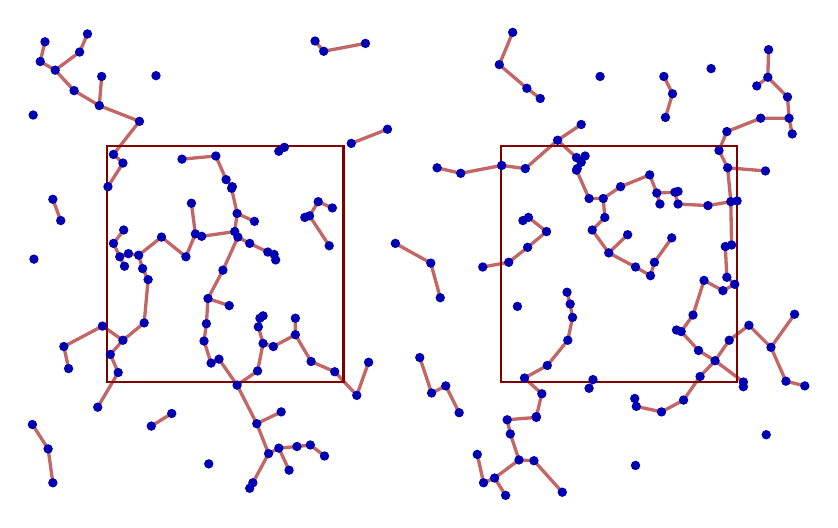
\begin{tikzpicture}[>=stealth]
    \tikzset{dot/.style={circle, fill=blue!70!black, inner sep=1.2pt, outer sep=0pt}}
    \tikzset{edge/.style={line width=1.2pt, red!60!black, opacity=0.6}}
    \tikzset{sq/.style={thick, red!50!black}}

    \draw[sq] (1.0, 1.5) rectangle (4.0, 4.5);
    \draw[sq] (6.0, 1.5) rectangle (9.0, 4.5);
      \draw[edge] (3.75,5.70)--(3.64,5.83) (3.75,5.70)--(4.28,5.80) (7.32,3.59)--(7.30,3.83) (7.32,3.59)--(7.16,3.43) (1.56,0.94)--(1.82,1.10) (0.58,5.20)--(0.34,5.46) (0.58,5.20)--(0.90,5.01) (6.01,4.25)--(5.49,4.15) (6.01,4.25)--(6.31,4.21) (0.21,5.82)--(0.15,5.57) (8.32,1.27)--(8.04,1.12) (8.32,1.27)--(8.53,1.57) (3.04,3.15)--(3.12,3.12) (3.04,3.15)--(2.81,3.26) (4.32,1.75)--(4.17,1.33) (6.12,0.84)--(6.08,1.02) (6.12,0.84)--(6.23,0.51) (2.92,2.20)--(2.94,2.31) (2.92,2.20)--(2.98,1.99) (4.56,4.71)--(4.10,4.53) (2.00,3.09)--(1.69,3.34) (2.00,3.09)--(2.12,3.38) (5.92,0.28)--(6.06,0.06) (5.92,0.28)--(5.78,0.22) (5.92,0.28)--(6.23,0.51) (6.08,1.02)--(6.45,1.05) (0.65,5.69)--(0.34,5.46) (0.65,5.69)--(0.75,5.92) (9.66,4.85)--(9.70,4.65) (9.66,4.85)--(9.30,4.85) (9.66,4.85)--(9.64,5.12) (3.05,0.59)--(2.90,0.97) (3.05,0.59)--(3.18,0.66) (3.05,0.59)--(2.85,0.22) (6.84,2.64)--(6.88,2.49) (1.22,2.97)--(1.16,3.09) (0.34,5.46)--(0.15,5.57) (2.59,3.98)--(2.58,3.96) (2.59,3.98)--(2.51,4.07) (3.12,3.12)--(3.14,3.05) (5.47,1.11)--(5.30,1.45) (9.39,5.37)--(9.25,5.26) (9.39,5.37)--(9.40,5.72) (9.39,5.37)--(9.64,5.12) (5.98,5.53)--(6.33,5.23) (5.98,5.53)--(6.15,5.94) (0.88,1.18)--(1.14,1.62) (0.45,1.95)--(0.51,1.67) (0.45,1.95)--(0.94,2.21) (3.89,1.63)--(4.17,1.33);
      \draw[edge] (3.89,1.63)--(3.59,1.76) (8.29,2.14)--(8.51,1.90) (8.29,2.14)--(8.23,2.16) (8.29,2.14)--(8.44,2.35) (2.81,3.26)--(2.66,3.34) (1.41,4.81)--(0.90,5.01) (1.41,4.81)--(1.08,4.39) (7.72,1.19)--(8.04,1.12) (7.72,1.19)--(7.70,1.29) (7.07,4.37)--(7.02,4.29) (3.58,0.70)--(3.41,0.68) (3.58,0.70)--(3.76,0.56) (8.63,3.74)--(8.92,3.79) (8.63,3.74)--(8.25,3.76) (3.31,0.38)--(3.18,0.66) (3.11,1.95)--(3.39,2.10) (3.11,1.95)--(2.98,1.99) (7.30,3.83)--(7.12,3.83) (7.30,3.83)--(7.52,3.98) (8.87,2.83)--(8.97,2.74) (8.87,2.83)--(8.85,3.22) (1.20,4.28)--(1.01,3.98) (1.20,4.28)--(1.08,4.39) (7.61,3.37)--(7.37,3.14) (7.71,2.96)--(7.37,3.14) (7.71,2.96)--(7.90,2.85) (5.23,2.57)--(5.11,3.01) (0.25,0.65)--(0.05,0.96) (0.25,0.65)--(0.31,0.22) (0.31,3.82)--(0.41,3.55) (9.08,1.50)--(9.08,1.44) (9.08,1.50)--(8.72,1.77) (2.90,0.97)--(3.21,1.12) (2.90,0.97)--(2.65,1.46) (9.30,4.85)--(8.87,4.68) (6.33,5.23)--(6.50,5.10) (8.93,3.24)--(8.92,3.79) (8.93,3.24)--(8.85,3.22) (8.07,5.38)--(8.18,5.16) (3.18,0.66)--(3.41,0.68) (2.28,2.56)--(2.55,2.47) (2.28,2.56)--(2.26,2.24) (2.28,2.56)--(2.47,2.92) (8.18,5.16)--(8.09,4.86) (1.20,2.03)--(0.94,2.21) (1.20,2.03)--(1.47,2.25) (1.20,2.03)--(1.04,1.85) (9.43,1.94)--(9.62,1.51) (9.43,1.94)--(9.73,2.36) (9.43,1.94)--(9.15,2.22);
      \draw[edge] (5.19,4.22)--(5.49,4.15) (9.62,1.51)--(9.86,1.45) (4.97,1.81)--(5.12,1.36) (2.85,0.22)--(2.81,0.15) (6.10,3.02)--(6.34,3.21) (6.10,3.02)--(5.77,2.96) (1.45,2.94)--(1.40,3.11) (1.45,2.94)--(1.52,2.80) (6.72,4.57)--(7.02,4.77) (6.72,4.57)--(6.31,4.21) (6.72,4.57)--(6.96,4.35) (2.38,4.37)--(1.95,4.33) (2.38,4.37)--(2.51,4.07) (3.68,3.79)--(3.86,3.71) (3.68,3.79)--(3.57,3.61) (6.34,3.21)--(6.58,3.41) (0.90,5.01)--(0.93,5.38) (6.78,0.10)--(6.42,0.50) (5.12,1.36)--(5.30,1.45) (6.45,1.05)--(6.45,1.06) (6.91,2.32)--(6.85,2.03) (6.91,2.32)--(6.88,2.49) (2.58,3.96)--(2.65,3.64) (8.17,3.33)--(7.95,3.02) (9.00,3.80)--(8.92,3.79) (3.39,2.10)--(3.59,1.76) (3.39,2.10)--(3.39,2.31) (8.87,4.68)--(8.77,4.44) (6.42,0.50)--(6.23,0.51) (6.52,1.35)--(6.45,1.06) (6.52,1.35)--(6.30,1.55) (7.12,1.42)--(7.17,1.53) (3.25,4.48)--(3.18,4.43) (6.58,3.41)--(6.35,3.59) (2.65,1.46)--(2.42,1.79) (2.65,1.46)--(2.91,1.64) (8.92,3.79)--(8.88,4.22) (7.95,3.02)--(7.90,2.85) (9.15,2.22)--(8.90,2.03) (2.94,2.31)--(2.98,2.34) (8.51,1.90)--(8.72,1.77) (1.69,3.34)--(1.40,3.11) (9.36,4.18)--(8.88,4.22) (5.70,0.58)--(5.78,0.22) (1.40,3.11)--(1.27,3.13) (8.77,4.44)--(8.88,4.22) (6.97,4.21)--(7.02,4.29) (6.97,4.21)--(6.96,4.19) (5.11,3.01)--(4.66,3.26) (7.98,3.90)--(7.89,4.13);
      \draw[edge] (7.98,3.90)--(8.21,3.91) (7.98,3.90)--(8.02,3.76) (8.90,2.03)--(8.72,1.77) (2.87,3.54)--(2.65,3.64) (1.27,3.13)--(1.16,3.09) (1.16,3.09)--(1.08,3.26) (2.62,3.41)--(2.65,3.64) (2.62,3.41)--(2.66,3.34) (2.62,3.41)--(2.20,3.35) (2.32,1.74)--(2.23,2.02) (2.32,1.74)--(2.42,1.79) (3.51,3.59)--(3.57,3.61) (2.23,2.02)--(2.26,2.24) (1.47,2.25)--(1.52,2.80) (2.66,3.34)--(2.47,2.92) (2.07,3.77)--(2.12,3.38) (1.04,1.85)--(1.14,1.62) (3.57,3.61)--(3.82,3.23) (2.20,3.35)--(2.12,3.38) (2.91,1.64)--(2.98,1.99) (1.21,3.43)--(1.08,3.26) (7.16,3.43)--(7.37,3.14) (8.82,2.66)--(8.97,2.74) (8.82,2.66)--(8.58,2.79) (6.59,1.71)--(6.30,1.55) (6.59,1.71)--(6.85,2.03) (6.28,3.55)--(6.35,3.59) (8.53,1.57)--(8.72,1.77) (8.44,2.35)--(8.58,2.79) (7.89,4.13)--(7.52,3.98) (8.21,3.91)--(8.25,3.92) (8.21,3.91)--(8.25,3.76) (7.12,3.83)--(6.96,4.19) (7.02,4.29)--(6.96,4.35);
    \foreach \x/\y in {3.75/5.70, 7.32/3.59, 1.56/0.94, 0.58/5.20, 6.01/4.25, 0.21/5.82, 8.32/1.27, 1.82/1.10, 3.04/3.15, 4.32/1.75, 6.12/0.84, 2.92/2.20, 4.56/4.71, 2.00/3.09, 5.92/0.28, 6.08/1.02, 0.65/5.69, 9.66/4.85, 3.05/0.59, 6.84/2.64, 1.22/2.97, 0.34/5.46, 2.59/3.98, 3.12/3.12, 5.47/1.11, 9.70/4.65, 9.39/5.37, 5.98/5.53, 0.88/1.18, 0.45/1.95, 3.89/1.63, 8.29/2.14, 2.81/3.26, 1.41/4.81, 0.75/5.92, 7.72/1.19, 0.06/4.89, 7.07/4.37, 7.71/0.44, 3.58/0.70, 8.63/3.74, 3.31/0.38, 3.11/1.95, 7.30/3.83, 8.87/2.83, 1.20/4.28, 7.61/3.37, 7.71/2.96, 5.23/2.57, 0.25/0.65, 0.31/3.82, 3.14/3.05, 9.08/1.50, 4.10/4.53, 2.29/0.46, 2.90/0.97, 9.30/4.85, 6.33/5.23, 8.04/1.12, 8.93/3.24, 8.07/5.38, 3.18/0.66, 2.28/2.56, 8.18/5.16, 0.07/3.06, 4.17/1.33, 1.20/2.03, 9.43/1.94, 5.19/4.22, 3.64/5.83, 9.62/1.51, 4.97/1.81, 2.85/0.22, 6.10/3.02, 0.51/1.67, 9.08/1.44, 1.45/2.94, 9.86/1.45, 6.72/4.57, 2.38/4.37, 3.68/3.79, 6.34/3.21, 0.90/5.01, 3.21/1.12, 0.41/3.55, 6.78/0.10, 5.12/1.36, 6.45/1.05, 6.91/2.32, 9.37/0.83, 3.41/0.68, 9.25/5.26, 2.58/3.96, 8.17/3.33, 5.30/1.45, 0.93/5.38, 9.00/3.80, 3.39/2.10, 7.26/5.38, 8.87/4.68, 6.42/0.50, 1.62/5.39, 6.06/0.06, 1.01/3.98, 0.05/0.96, 5.49/4.15, 6.52/1.35, 7.12/1.42, 3.25/4.48, 6.50/5.10, 6.58/3.41, 0.94/2.21, 2.65/1.46, 9.73/2.36, 8.92/3.79, 7.95/3.02, 5.77/2.96, 1.95/4.33, 2.81/0.15, 6.45/1.06, 9.40/5.72, 9.15/2.22, 0.15/5.57, 4.28/5.80, 9.64/5.12, 2.94/2.31, 8.51/1.90, 1.69/3.34, 9.36/4.18, 5.70/0.58, 6.15/5.94, 1.40/3.11, 8.77/4.44, 6.97/4.21, 3.59/1.76, 8.09/4.86, 8.67/5.48, 5.11/3.01, 7.98/3.90, 7.02/4.77, 8.90/2.03, 3.76/0.56, 5.78/0.22, 4.66/3.26, 2.87/3.54, 0.31/0.22, 8.23/2.16, 1.27/3.13, 7.70/1.29, 6.23/0.51, 1.16/3.09, 2.62/3.41, 3.18/4.43, 2.55/2.47, 3.39/2.31, 2.32/1.74, 1.08/4.39, 3.51/3.59, 2.23/2.02, 1.47/2.25, 2.65/3.64, 2.98/2.34, 3.86/3.71, 2.66/3.34, 2.26/2.24, 2.07/3.77, 1.04/1.85, 1.14/1.62, 3.57/3.61, 2.42/1.79, 2.47/2.92, 1.52/2.80, 2.20/3.35, 2.91/1.64, 2.12/3.38, 2.51/4.07, 2.98/1.99, 1.21/3.43, 1.08/3.26, 3.82/3.23, 7.16/3.43, 7.37/3.14, 8.82/2.66, 8.88/4.22, 6.59/1.71, 6.30/1.55, 6.28/3.55, 6.21/2.46, 8.53/1.57, 8.44/2.35, 6.35/3.59, 7.89/4.13, 8.21/3.91, 6.85/2.03, 8.25/3.92, 8.97/2.74, 7.12/3.83, 7.02/4.29, 8.58/2.79, 8.25/3.76, 6.31/4.21, 7.52/3.98, 6.96/4.19, 7.17/1.53, 8.72/1.77, 6.96/4.35, 8.85/3.22, 7.90/2.85, 6.88/2.49, 8.02/3.76} {
        \node[dot] at (\x, \y) {};
    }
  \end{tikzpicture}
  }
  \caption{Arbre couvrant minimum élagué au rayon $r_1$. La percolation a eu lieu sur les deux carrés de forte densité mais pas sur le fond.}
  \label{fig:mst_r1}
\end{subfigure}
\hfill
\begin{subfigure}[b]{0.48\textwidth}
  \resizebox{\linewidth}{!}{
  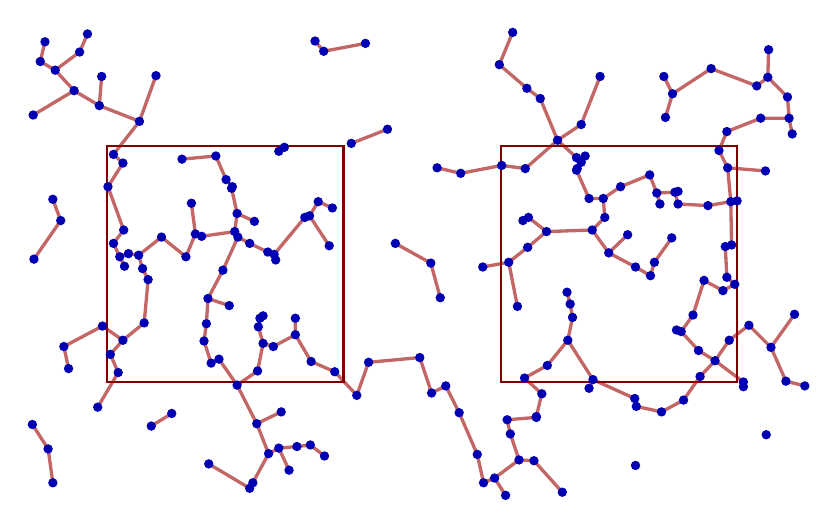
\begin{tikzpicture}[>=stealth]
    \tikzset{dot/.style={circle, fill=blue!70!black, inner sep=1.2pt, outer sep=0pt}}
    \tikzset{edge/.style={line width=1.2pt, red!60!black, opacity=0.6}}
    \tikzset{sq/.style={thick, red!50!black}}

    \draw[sq] (1.0, 1.5) rectangle (4.0, 4.5);
    \draw[sq] (6.0, 1.5) rectangle (9.0, 4.5);
      \draw[edge] (3.75,5.70)--(3.64,5.83) (3.75,5.70)--(4.28,5.80) (7.32,3.59)--(7.30,3.83) (7.32,3.59)--(7.16,3.43) (1.56,0.94)--(1.82,1.10) (0.58,5.20)--(0.34,5.46) (0.58,5.20)--(0.06,4.89) (0.58,5.20)--(0.90,5.01) (6.01,4.25)--(5.49,4.15) (6.01,4.25)--(6.31,4.21) (0.21,5.82)--(0.15,5.57) (8.32,1.27)--(8.04,1.12) (8.32,1.27)--(8.53,1.57) (3.04,3.15)--(3.12,3.12) (3.04,3.15)--(2.81,3.26) (4.32,1.75)--(4.17,1.33) (4.32,1.75)--(4.97,1.81) (6.12,0.84)--(6.08,1.02) (6.12,0.84)--(6.23,0.51) (2.92,2.20)--(2.94,2.31) (2.92,2.20)--(2.98,1.99) (4.56,4.71)--(4.10,4.53) (2.00,3.09)--(1.69,3.34) (2.00,3.09)--(2.12,3.38) (5.92,0.28)--(6.06,0.06) (5.92,0.28)--(5.78,0.22) (5.92,0.28)--(6.23,0.51) (6.08,1.02)--(6.45,1.05) (0.65,5.69)--(0.34,5.46) (0.65,5.69)--(0.75,5.92) (9.66,4.85)--(9.70,4.65) (9.66,4.85)--(9.30,4.85) (9.66,4.85)--(9.64,5.12) (3.05,0.59)--(2.90,0.97) (3.05,0.59)--(3.18,0.66) (3.05,0.59)--(2.85,0.22) (6.84,2.64)--(6.88,2.49) (1.22,2.97)--(1.16,3.09) (0.34,5.46)--(0.15,5.57) (2.59,3.98)--(2.58,3.96) (2.59,3.98)--(2.51,4.07) (3.12,3.12)--(3.14,3.05) (3.12,3.12)--(3.51,3.59) (5.47,1.11)--(5.30,1.45) (5.47,1.11)--(5.70,0.58) (9.39,5.37)--(9.25,5.26) (9.39,5.37)--(9.40,5.72) (9.39,5.37)--(9.64,5.12) (5.98,5.53)--(6.33,5.23) (5.98,5.53)--(6.15,5.94);
      \draw[edge] (0.88,1.18)--(1.14,1.62) (0.45,1.95)--(0.51,1.67) (0.45,1.95)--(0.94,2.21) (3.89,1.63)--(4.17,1.33) (3.89,1.63)--(3.59,1.76) (8.29,2.14)--(8.51,1.90) (8.29,2.14)--(8.23,2.16) (8.29,2.14)--(8.44,2.35) (2.81,3.26)--(2.66,3.34) (1.41,4.81)--(0.90,5.01) (1.41,4.81)--(1.62,5.39) (1.41,4.81)--(1.08,4.39) (7.72,1.19)--(8.04,1.12) (7.72,1.19)--(7.70,1.29) (7.07,4.37)--(7.02,4.29) (3.58,0.70)--(3.41,0.68) (3.58,0.70)--(3.76,0.56) (8.63,3.74)--(8.92,3.79) (8.63,3.74)--(8.25,3.76) (3.31,0.38)--(3.18,0.66) (3.11,1.95)--(3.39,2.10) (3.11,1.95)--(2.98,1.99) (7.30,3.83)--(7.12,3.83) (7.30,3.83)--(7.52,3.98) (8.87,2.83)--(8.97,2.74) (8.87,2.83)--(8.85,3.22) (1.20,4.28)--(1.01,3.98) (1.20,4.28)--(1.08,4.39) (7.61,3.37)--(7.37,3.14) (7.71,2.96)--(7.37,3.14) (7.71,2.96)--(7.90,2.85) (5.23,2.57)--(5.11,3.01) (0.25,0.65)--(0.05,0.96) (0.25,0.65)--(0.31,0.22) (0.31,3.82)--(0.41,3.55) (9.08,1.50)--(9.08,1.44) (9.08,1.50)--(8.72,1.77) (2.29,0.46)--(2.81,0.15) (2.90,0.97)--(3.21,1.12) (2.90,0.97)--(2.65,1.46) (9.30,4.85)--(8.87,4.68) (6.33,5.23)--(6.50,5.10) (8.93,3.24)--(8.92,3.79) (8.93,3.24)--(8.85,3.22) (8.07,5.38)--(8.18,5.16) (3.18,0.66)--(3.41,0.68) (2.28,2.56)--(2.55,2.47) (2.28,2.56)--(2.26,2.24) (2.28,2.56)--(2.47,2.92) (8.18,5.16)--(8.09,4.86);
      \draw[edge] (8.18,5.16)--(8.67,5.48) (0.07,3.06)--(0.41,3.55) (1.20,2.03)--(0.94,2.21) (1.20,2.03)--(1.47,2.25) (1.20,2.03)--(1.04,1.85) (9.43,1.94)--(9.62,1.51) (9.43,1.94)--(9.73,2.36) (9.43,1.94)--(9.15,2.22) (5.19,4.22)--(5.49,4.15) (9.62,1.51)--(9.86,1.45) (4.97,1.81)--(5.12,1.36) (2.85,0.22)--(2.81,0.15) (6.10,3.02)--(6.34,3.21) (6.10,3.02)--(5.77,2.96) (6.10,3.02)--(6.21,2.46) (1.45,2.94)--(1.40,3.11) (1.45,2.94)--(1.52,2.80) (6.72,4.57)--(6.50,5.10) (6.72,4.57)--(7.02,4.77) (6.72,4.57)--(6.31,4.21) (6.72,4.57)--(6.96,4.35) (2.38,4.37)--(1.95,4.33) (2.38,4.37)--(2.51,4.07) (3.68,3.79)--(3.86,3.71) (3.68,3.79)--(3.57,3.61) (6.34,3.21)--(6.58,3.41) (0.90,5.01)--(0.93,5.38) (6.78,0.10)--(6.42,0.50) (5.12,1.36)--(5.30,1.45) (6.45,1.05)--(6.45,1.06) (6.91,2.32)--(6.85,2.03) (6.91,2.32)--(6.88,2.49) (9.25,5.26)--(8.67,5.48) (2.58,3.96)--(2.65,3.64) (8.17,3.33)--(7.95,3.02) (9.00,3.80)--(8.92,3.79) (3.39,2.10)--(3.59,1.76) (3.39,2.10)--(3.39,2.31) (7.26,5.38)--(7.02,4.77) (8.87,4.68)--(8.77,4.44) (6.42,0.50)--(6.23,0.51) (1.01,3.98)--(1.21,3.43) (6.52,1.35)--(6.45,1.06) (6.52,1.35)--(6.30,1.55) (7.12,1.42)--(7.17,1.53) (3.25,4.48)--(3.18,4.43) (6.58,3.41)--(7.16,3.43) (6.58,3.41)--(6.35,3.59) (2.65,1.46)--(2.42,1.79) (2.65,1.46)--(2.91,1.64);
      \draw[edge] (8.92,3.79)--(8.88,4.22) (7.95,3.02)--(7.90,2.85) (9.15,2.22)--(8.90,2.03) (2.94,2.31)--(2.98,2.34) (8.51,1.90)--(8.72,1.77) (1.69,3.34)--(1.40,3.11) (9.36,4.18)--(8.88,4.22) (5.70,0.58)--(5.78,0.22) (1.40,3.11)--(1.27,3.13) (8.77,4.44)--(8.88,4.22) (6.97,4.21)--(7.02,4.29) (6.97,4.21)--(6.96,4.19) (5.11,3.01)--(4.66,3.26) (7.98,3.90)--(7.89,4.13) (7.98,3.90)--(8.21,3.91) (7.98,3.90)--(8.02,3.76) (8.90,2.03)--(8.72,1.77) (2.87,3.54)--(2.65,3.64) (1.27,3.13)--(1.16,3.09) (7.70,1.29)--(7.17,1.53) (1.16,3.09)--(1.08,3.26) (2.62,3.41)--(2.65,3.64) (2.62,3.41)--(2.66,3.34) (2.62,3.41)--(2.20,3.35) (2.32,1.74)--(2.23,2.02) (2.32,1.74)--(2.42,1.79) (3.51,3.59)--(3.57,3.61) (2.23,2.02)--(2.26,2.24) (1.47,2.25)--(1.52,2.80) (2.66,3.34)--(2.47,2.92) (2.07,3.77)--(2.12,3.38) (1.04,1.85)--(1.14,1.62) (3.57,3.61)--(3.82,3.23) (2.20,3.35)--(2.12,3.38) (2.91,1.64)--(2.98,1.99) (1.21,3.43)--(1.08,3.26) (7.16,3.43)--(7.37,3.14) (8.82,2.66)--(8.97,2.74) (8.82,2.66)--(8.58,2.79) (6.59,1.71)--(6.30,1.55) (6.59,1.71)--(6.85,2.03) (6.28,3.55)--(6.35,3.59) (8.53,1.57)--(8.72,1.77) (8.44,2.35)--(8.58,2.79) (7.89,4.13)--(7.52,3.98) (8.21,3.91)--(8.25,3.92) (8.21,3.91)--(8.25,3.76) (6.85,2.03)--(7.17,1.53) (7.12,3.83)--(6.96,4.19) (7.02,4.29)--(6.96,4.35);
    \foreach \x/\y in {3.75/5.70, 7.32/3.59, 1.56/0.94, 0.58/5.20, 6.01/4.25, 0.21/5.82, 8.32/1.27, 1.82/1.10, 3.04/3.15, 4.32/1.75, 6.12/0.84, 2.92/2.20, 4.56/4.71, 2.00/3.09, 5.92/0.28, 6.08/1.02, 0.65/5.69, 9.66/4.85, 3.05/0.59, 6.84/2.64, 1.22/2.97, 0.34/5.46, 2.59/3.98, 3.12/3.12, 5.47/1.11, 9.70/4.65, 9.39/5.37, 5.98/5.53, 0.88/1.18, 0.45/1.95, 3.89/1.63, 8.29/2.14, 2.81/3.26, 1.41/4.81, 0.75/5.92, 7.72/1.19, 0.06/4.89, 7.07/4.37, 7.71/0.44, 3.58/0.70, 8.63/3.74, 3.31/0.38, 3.11/1.95, 7.30/3.83, 8.87/2.83, 1.20/4.28, 7.61/3.37, 7.71/2.96, 5.23/2.57, 0.25/0.65, 0.31/3.82, 3.14/3.05, 9.08/1.50, 4.10/4.53, 2.29/0.46, 2.90/0.97, 9.30/4.85, 6.33/5.23, 8.04/1.12, 8.93/3.24, 8.07/5.38, 3.18/0.66, 2.28/2.56, 8.18/5.16, 0.07/3.06, 4.17/1.33, 1.20/2.03, 9.43/1.94, 5.19/4.22, 3.64/5.83, 9.62/1.51, 4.97/1.81, 2.85/0.22, 6.10/3.02, 0.51/1.67, 9.08/1.44, 1.45/2.94, 9.86/1.45, 6.72/4.57, 2.38/4.37, 3.68/3.79, 6.34/3.21, 0.90/5.01, 3.21/1.12, 0.41/3.55, 6.78/0.10, 5.12/1.36, 6.45/1.05, 6.91/2.32, 9.37/0.83, 3.41/0.68, 9.25/5.26, 2.58/3.96, 8.17/3.33, 5.30/1.45, 0.93/5.38, 9.00/3.80, 3.39/2.10, 7.26/5.38, 8.87/4.68, 6.42/0.50, 1.62/5.39, 6.06/0.06, 1.01/3.98, 0.05/0.96, 5.49/4.15, 6.52/1.35, 7.12/1.42, 3.25/4.48, 6.50/5.10, 6.58/3.41, 0.94/2.21, 2.65/1.46, 9.73/2.36, 8.92/3.79, 7.95/3.02, 5.77/2.96, 1.95/4.33, 2.81/0.15, 6.45/1.06, 9.40/5.72, 9.15/2.22, 0.15/5.57, 4.28/5.80, 9.64/5.12, 2.94/2.31, 8.51/1.90, 1.69/3.34, 9.36/4.18, 5.70/0.58, 6.15/5.94, 1.40/3.11, 8.77/4.44, 6.97/4.21, 3.59/1.76, 8.09/4.86, 8.67/5.48, 5.11/3.01, 7.98/3.90, 7.02/4.77, 8.90/2.03, 3.76/0.56, 5.78/0.22, 4.66/3.26, 2.87/3.54, 0.31/0.22, 8.23/2.16, 1.27/3.13, 7.70/1.29, 6.23/0.51, 1.16/3.09, 2.62/3.41, 3.18/4.43, 2.55/2.47, 3.39/2.31, 2.32/1.74, 1.08/4.39, 3.51/3.59, 2.23/2.02, 1.47/2.25, 2.65/3.64, 2.98/2.34, 3.86/3.71, 2.66/3.34, 2.26/2.24, 2.07/3.77, 1.04/1.85, 1.14/1.62, 3.57/3.61, 2.42/1.79, 2.47/2.92, 1.52/2.80, 2.20/3.35, 2.91/1.64, 2.12/3.38, 2.51/4.07, 2.98/1.99, 1.21/3.43, 1.08/3.26, 3.82/3.23, 7.16/3.43, 7.37/3.14, 8.82/2.66, 8.88/4.22, 6.59/1.71, 6.30/1.55, 6.28/3.55, 6.21/2.46, 8.53/1.57, 8.44/2.35, 6.35/3.59, 7.89/4.13, 8.21/3.91, 6.85/2.03, 8.25/3.92, 8.97/2.74, 7.12/3.83, 7.02/4.29, 8.58/2.79, 8.25/3.76, 6.31/4.21, 7.52/3.98, 6.96/4.19, 7.17/1.53, 8.72/1.77, 6.96/4.35, 8.85/3.22, 7.90/2.85, 6.88/2.49, 8.02/3.76} {
        \node[dot] at (\x, \y) {};
    }
  \end{tikzpicture}
  }
  \caption{Arbre couvrant minimum élagué au rayon $r_2 > r_1$, de sorte que la percolation a eu lieu partout.}
  \label{fig:mst_r2}
\end{subfigure}

  }{%
    \fbox{\parbox{0.75\textwidth}{\centering Figure à générer : deux amas denses séparés par un fond de faible densité ; apparition des composantes géantes dans les amas puis fusion par percolation du fond.}}
  }
  \caption{Inconsistance du Single-Linkage en dimension $p\ge2$. Les deux amas de forte densité (carrés) sont fusionnés (droite, niveau $r_2$) avant que tous les points en faisant partie soient récupérés par les deux composantes géantes (gauche, niveau $r_1$).\label{fig:percolation_2_carres}}
\end{figure}

\subsection{Lecture générale avec la densité $f$}

Soit $\mathcal X_n$ un $n$-échantillon i.i.d. de densité $f$ dans $\mathbb R^p$, et soit $r_n\to0$ une échelle locale. Par rapport à notre normalisation $r=1/2$, autour d'un point $x$ où $f$ est régulière, le nuage vu à l'échelle $r_n$ ressemble à un processus de \textsc{Poisson} homogène d'intensité
\[
    \lambda_n(x) \simeq n(2r_n)^p f(x),
\]
Autrement dit, la fonction
\[
    \Theta^{\mathrm{fam}}_{K,p,1/2}
\]
donne la probabilité asymptotique qu'un point situé dans une région de densité $f(x)$ appartienne à la composante géante observée à cette échelle.

Pour une densité générale, la séparation entre deux amas dépend alors de la géométrie des cols et des vallées de $f$. 
Soit $C$ un amas de forte densité, c'est-à-dire une composante connexe de $H_f(\lambda)$ et $\tau < \lambda$ une densité plus faible pour laquelle une vallée de plus faible densité, si elle devenait supercritique et percolait, ferait ``disparaître'' $C$ par fusion.
Juste avant cette fusion, la proportion récupérable de l'amas $C$ est heuristiquement donnée par la moyenne pondérée
\begin{equation}\label{eq:frac_recouvrement}
    \frac{
        \displaystyle \int_C
        \Theta^{\mathrm{fam}}_{K,p,1/2}
        \left(
            \lambda_c^{\mathrm{fam}}(K,p)\frac{f(x)}{\tau}
        \right)
        f(x)\,\mathrm dx
    }{
        \displaystyle \int_C f(x)\,\mathrm dx
    }.
\end{equation}

Le cas constant par morceaux ci-dessous est la version plus lisible de cette idée et qui permet de calculer un indice concret, la \emph{vitesse de percolation} (\Def~\ref{def:vitesse_critique}).

\subsection{Le cas simple des niveaux de densité constants}

Considérons deux domaines $A,B\subset\mathbb R^p$ compacts réguliers (connexes, avec $\overline{\mathring{A}} = A$ et $\partial A$ de $p$-mesure de Lebesgue nulle, \emph{idem} pour $B$), séparés par un domaine de fond $F \supset A \cup B$ contenant un corridor macroscopique (la dilatation d'un chemin lisse) reliant $A$ à $B$. Par souci de simplicité du modèle, on supposera que les données sont tirées selon une densité constante par morceaux :
\[
    f(x)=
    \rho\mathbf 1_{A\cup B}(x)+\rho_0\mathbf 1_F(x),
\]
où $\rho, \rho_0 > 0$. Posons
\[
    \rho_1 \eqdef \rho+\rho_0.
\]
Les ensembles $A$ et $B$ ont donc densité $\rho_1>\rho_0$ ; ce sont des amas de forte densité par rapport à la vallée de faible densité les reliant, à savoir $F \setminus (A\cup B)$. Voir la \Fig~\ref{fig:percolation_2_carres} pour une illustration : $A$ et $B$ sont les deux carrés inclus dans un long rectangle, le fond $F$.

\begin{Fait}{Fusion asymptotique lorsque le fond devient supercritique}{fusion_fond_supercritique}
Soit $\mathrm{fam}$ une famille de composantes parmi celles considérées ci-dessus, et soit $\lambda_c^{\mathrm{fam}}(K,p)$ son seuil critique. Supposons que le rayon $r_n$ soit choisi de sorte que le fond soit strictement supercritique :
\[
    n(2r_n)^p\rho_0
    >
    \lambda_c^{\mathrm{fam}}(K,p)+\eta
\]
pour un $\eta>0$ fixé. Alors, conditionnellement à l'existence de composantes géantes dans $A$ et $B$ atteignant les bords faisant face au corridor, ces deux composantes fusionnent avec probabilité tendant vers $1$ lorsque $n\to+\infty$.
\end{Fait}

\begin{Preuve}
Après changement d'échelle par $r_n$, le corridor contenu dans $F$ devient une boîte dont les dimensions tendent vers l'infini. Dans cette boîte, le processus de points converge localement vers un processus de \textsc{Poisson} homogène d'intensité normalisée strictement supérieure au seuil critique. Les résultats standards de percolation continue supercritique donnent alors l'existence, avec probabilité tendant vers $1$, d'une composante traversante reliant les deux faces opposées du corridor \cite{MeesterRoy, penrose2003}.

%L'hypothèse conditionnelle de l'énoncé sert précisément à ne pas ouvrir ici la question des estimées de traversée dans les deux amas compacts. Sous des hypothèses géométriques légèrement plus fortes sur $A$ et $B$ (par exemple la présence de boîtes macroscopiques accolées aux extrémités du corridor), cette hypothèse peut être remplacée par les estimées usuelles de traversée en régime supercritique \cite{MeesterRoy, penrose2003}.
\end{Preuve}

\begin{Theoreme}{Fraction récupérable avant fusion parasite}{fraction_recuperable}
Soit $\mathrm{fam}$ une méthode de clustering persistant, de probabilité de percolation $\Theta^{\mathrm{fam}}$ et de seuil critique $\lambda_c^{\mathrm{fam}}$. Dans le modèle à deux densités ci-dessus, la fraction asymptotiquement récupérable dans $A$ et $B$ juste avant la percolation du fond est
\[
    \Theta^{\mathrm{fam}}_{K,p,1/2}\left(
        \lambda_c^{\mathrm{fam}}(K,p)\frac{\rho_1}{\rho_0}
    \right).
\]
En particulier, un rappel asymptotique d'au moins $1-\varepsilon$ avant fusion parasite est possible si et seulement si
\[
    \frac{\rho_0}{\rho_1}
    \le
    \frac{\lambda_c^{\mathrm{fam}}(K,p)}
         {\lambda^{\mathrm{fam}}_{1-\varepsilon}(K,p)},
\]
où
\[
    \lambda^{\mathrm{fam}}_{1-\varepsilon}(K,p)
    \eqdef
    \inf\left\{\lambda>0:
    \Theta^{\mathrm{fam}}_{K,p,1/2}(\lambda)\ge 1-\varepsilon
    \right\}.
\]
\end{Theoreme}

\begin{Preuve}[\textsc{Preuve du \Th~\ref{th:fraction_recuperable}}]
À la limite où le fond devient critique (lorsque son intensité normalisée tend vers $\lambda_c^{\mathrm{fam}}(K,p)$ par valeurs supérieures), l'intensité normalisée dans $F$ vaut $\lambda_c^{\mathrm{fam}}(K,p)$. À cette même échelle, l'intensité normalisée dans $A$ et $B$ vaut
\[
    \lambda_c^{\mathrm{fam}}(K,p)\frac{\rho_1}{\rho_0}.
\]
La proportion de points appartenant à la composante géante dans un domaine homogène de cette intensité converge vers la probabilité de \textsc{Palm} correspondante (en supposant la continuité en ce point de la fonction), c'est-à-dire vers
\[
    \Theta^{\mathrm{fam}}_{K,p,1/2}\left(
        \lambda_c^{\mathrm{fam}}(K,p)\frac{\rho_1}{\rho_0}
    \right).
\]
Pour que cette quantité soit au moins $1-\varepsilon$, il faut et il suffit que
\[
    \frac{\rho_0}{\rho_1}
    \le
    \frac{\lambda_c^{\mathrm{fam}}(K,p)}
         {\lambda^{\mathrm{fam}}_{1-\varepsilon}(K,p)},
\]
ce qui donne exactement l'inégalité annoncée.
\end{Preuve}


\section{La \emph{vitesse de percolation}}

Le \Th~\ref{th:fraction_recuperable} précédent motive la définition suivante.

\begin{Definition}{Vitesse critique de percolation}{vitesse_critique}
Pour une famille $\mathrm{fam}$, on définit le quantile de rappel au niveau $\alpha \in [ 0 ; 1]$
\[
    \lambda^{\mathrm{fam}}_{\alpha}(K,p)
    \eqdef
    \inf\left\{
        \lambda>0 \, \mid \,
        \Theta^{\mathrm{fam}}_{K,p,1/2}(\lambda)
        \ge \alpha
    \right\}.
\]
La \emph{vitesse critique de percolation} est le rapport
\[
    v^{\mathrm{fam}}_{\mathrm{crit},K,p}(\varepsilon)
    \eqdef
    \frac{
        \lambda_c^{\mathrm{fam}}(K,p)
    }{
        \lambda^{\mathrm{fam}}_{1-\varepsilon}(K,p)
    }.
\]
\end{Definition}

\Remarque{Plus cette quantité est proche de $1$, plus la méthode récupère rapidement une grande fraction d'un amas dense avant que le fond ne percole. C'est donc un indice de performance directement lisible sur la courbe $\Theta$.}

Le seuil critique $\lambda_c$ est en pratique difficile à estimer ; aussi l'avions-nous remplacé dans \cite{BibiIstambul} par le quantile de niveau $\varepsilon$ :
\[
    v^{\mathrm{fam}}_{K,p}(\varepsilon)
    \eqdef
    \frac{
        \lambda_\varepsilon^{\mathrm{fam}}(K,p)
    }{
        \lambda_{1-\varepsilon}^{\mathrm{fam}}(K,p)
    }.
\]


\Remarque{Si l'on préfère raisonner en rayons plutôt qu'en intensités, alors il suffit de remplacer dans la formule les quantiles des intensités par ceux des rayons
\[
    \frac{
        \lambda_\varepsilon^{\mathrm{fam}}(K,p)
    }{
        \lambda_{1-\varepsilon}^{\mathrm{fam}}(K,p)
    } =
        \left(\frac{
        r_\varepsilon^{\mathrm{fam}}(K,p)
    }{
        r_{1-\varepsilon}^{\mathrm{fam}}(K,p)
    }\right)^p.
\]
}


\section{Comparaison empirique entre $K$-polyèdres, $K$-Robust Single-Linkage et DBSCAN}

Les expériences de ce chapitre suivent le protocole suivant :
\begin{enumerate}
    \item Fixer $\mathrm{K\_list}$ une liste de $K$ possibles, la dimension $p \in \mathbb N^\star$, $T\gets 100$ le nombre de tests, $n\gets 100\,000$ le nombre de points et $\varepsilon \gets 3\%$.
    \item Pour $t \in \{1 ; \ldots ; T\}$ :
    \begin{enumerate}
        \item L'on génère $\mathcal X$ contenant $n$ points uniformément tirés dans l'hypercube $\left[0,n^{1/p}\right]^p$ (approximation \textsc{Poisson}/binomiale).
        \item Pour $\mathrm{fam} \in \{\mathrm{poly}, \mathrm{core}, \mathrm{DBSCAN}\}$, générer de façon efficace (voir chapitre suivant pour les $K$-polyèdres) la hiérarchie produite par $\mathrm{fam}$ sur $\mathcal X$ en repérant les rayons de fusion et la proportion de points se trouvant alors dans la plus grande composante connexe.
    \end{enumerate}
    \item En déduire un estimateur $\widehat{\Theta}^{\mathrm{fam}}$ de $\Theta^{\mathrm{fam}}$ ainsi que de la vitesse de percolation
    \[
    \widehat v^{\mathrm{fam}} \eqdef \frac{\widehat \lambda^{\mathrm{fam}}_{\varepsilon}}{\widehat \lambda^{\mathrm{fam}}_{1-\varepsilon}}.
    \]
\end{enumerate}

\Remarques{
\begin{enumerate}
    \item Lorsque $K=1$, les trois familles coïncident : les $1$-polyèdres sont les composantes du graphe géométrique, les points cœurs du $1$-Robust Single-Linkage sont tous les points qui apparaissent dans le modèle booléen, et DBSCAN ne fait qu'ajouter une frontière déjà présente. Les différences ne commencent donc qu'à partir de $K\ge2$.
    \item Pour $K=2$, le $K$-Robust Single-Linkage retire les feuilles des graphes géométriques mais n'identifie pas pour autant de structures plus fines. Cet élagage non nécessaire entraîne comme nous allons le voir des résultats pires que ceux de $K=1$. DBSCAN réajoute ensuite ces points accessibles (qui correspondent exactement aux feuilles élaguées) ; $K=2$ donne donc les mêmes résultats pour DBSCAN que $K=1$.
\end{enumerate}}

\begin{figure}[!h]
    \centering
        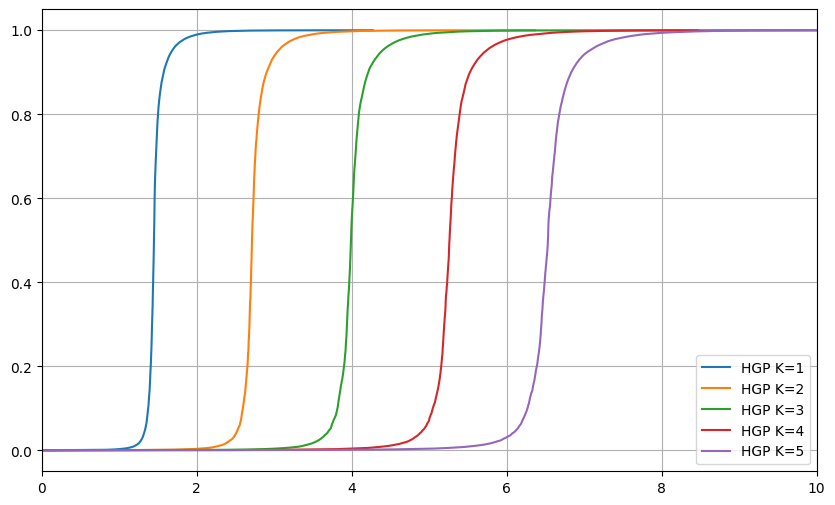
\includegraphics[width=0.7\textwidth]{img/vitesse_percolation_HGP_d2.png}
    \caption{Estimation de la fonction de probabilité $\lambda \mapsto \widehat \Theta^{\mathrm{poly}}_{K,2}(\lambda)$ pour $K \in \{1,2,3,4,5\}$ des $K$-polyèdres en dimension $2$. À noter que pour $K=1$, le seuil critique en 2D est $\lambda_c  \approx 1.44$ \cite{Quintanilla, lambdacR2}.\label{fig:Theta_HGP_d2}}
\end{figure}

\begin{figure}[!h]
    \centering
        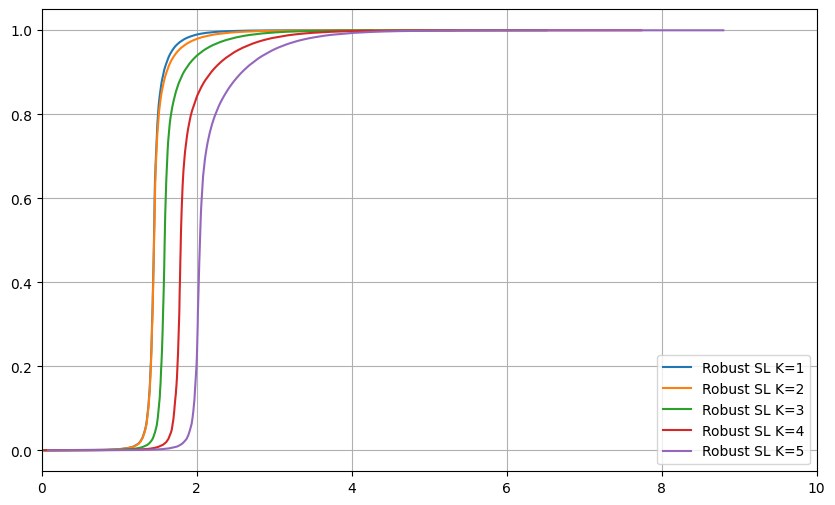
\includegraphics[width=0.7\textwidth]{img/vitesse_percolation_RSL_d2.png}
    \caption{Estimation de la fonction de probabilité $\lambda \mapsto \widehat \Theta^{\mathrm{core}}_{K,2}(\lambda)$ pour $K \in \{1,2,3,4,5\}$ des $K$-composantes du Robust Single-Linkage en dimension $2$.\label{fig:Theta_RSL_d2}}
\end{figure}

\begin{figure}[!h]
    \centering
        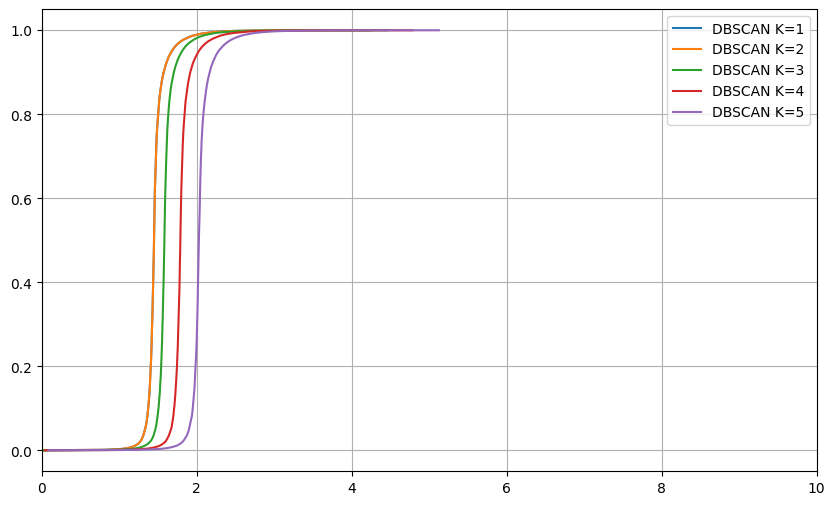
\includegraphics[width=0.7\textwidth]{img/vitesse_percolation_DBSCAN_d2.png}
    \caption{Estimation de la fonction de probabilité $\lambda \mapsto \widehat \Theta^{\mathrm{DBSCAN}}_{K,2}(\lambda)$ pour $K \in \{1,2,3,4,5\}$ des $K$-composantes de DBSCAN en dimension $2$.\label{fig:Theta_DBSCAN_d2}}
\end{figure}

\begin{table}[htbp]
    \centering
    \caption{\textcolor{red}{Ajouter $p=4$ ? }Vitesse de percolation $v$ en fonction de $K$ pour les dimensions $p=2$ et $p=3$. Les meilleurs résultats sont indiqués en gras.}
    \label{tab:percolation_horizontal}
    \begin{tabular}{@{} l ccc c ccc @{}}
        \toprule
        & \multicolumn{3}{c}{$p=2$} & \phantom{a} & \multicolumn{3}{c}{$p=3$} \\
        \cmidrule{2-4} \cmidrule{6-8}
        $K$ & HGP & Robust SL & DBSCAN && HGP & Robust SL & DBSCAN \\
        \midrule
        1 & \textbf{0.7347} & \textbf{0.7347} & \textbf{0.7347} && \textbf{0.5627} & \textbf{0.5627} & \textbf{0.5627} \\
        2 & \textbf{0.7793} & 0.6891 & 0.7347 && \textbf{0.6459} & 0.4616 & 0.5627 \\
        3 & \textbf{0.7997} & 0.6323 & 0.7530 && \textbf{0.6897} & 0.4116 & 0.5817 \\
        4 & \textbf{0.8168} & 0.5978 & 0.7672 && \textbf{0.7140} & 0.4001 & 0.6046 \\
        5 & \textbf{0.8261} & 0.5837 & 0.7785 && \textbf{0.7317} & 0.3988 & 0.6250 \\
        \bottomrule
    \end{tabular}
\end{table}

Les résultats des estimations de $\widehat \Theta^{\mathrm{fam}}$ (pour $p=2$, $K\in \bigl\{ 1 ; 2; 3 ; 4 ; 5\bigr\}$) sont montrés en \Fig~\ref{fig:Theta_HGP_d2} pour $\mathrm{fam} = \mathrm{poly}$, en \Fig~\ref{fig:Theta_RSL_d2} pour $\mathrm{fam} = \mathrm{core} $ et en \Fig~\ref{fig:Theta_DBSCAN_d2} pour $\mathrm{fam} = \mathrm{DBSCAN}$.

Pour le calcul des vitesses de percolation $\widehat v^{\mathrm{fam}}$ (en dimension $p=2$ et $p=3$), se reporter au \Tab~\ref{tab:percolation_horizontal}.

\Remarque{Ces simulations, quoique faisant intervenir $n=100000$ points, montrent des fonctions $\lambda \mapsto \Theta(\lambda)$ ``démarrant'' au-dessus de $0$ avec une pente nulle. Pourtant, au moins pour le Single-Linkage ($K=1$), il a été montré que la pente au niveau du seuil $\lambda_c$ est strictement positive \cite{Penrose2018, Penrose2018Correction, Duminil-CopinRaoufiTassionAHL} :
\[
\exists C > 0, \forall \lambda \ge \lambda_c, \ \ \ \Theta(\lambda) \ge C \left( \lambda - \lambda_c\right).
\]}

Les $K$-polyèdres améliorent systématiquement la vitesse de percolation dès que $K\ge2$ et surpassent les $K$-cœurs du Robust Single-Linkage et les $K$-composantes DBSCAN. 

L'on s'attendait à ce que le $K$-Robust Single-Linkage soit moins bon que DBSCAN et que, pour $K=2$, il donne de moins bons résultats que $K=1$. 
En fait, c'est pis que cela : pour $K\ge3$, le Robust Single-Linkage continue de dégrader considérablement les résultats par rapport au Single-Linkage. La raison à cela se lit en \Fig~\ref{fig:Theta_RSL_d2} : l'algorithme peine à rassembler les derniers points ; sa probabilité de percolation $\Theta^{\mathrm{core}}$ converge trop lentement vers $1$. L'erreur de ne pas prendre en compte les points à la frontière des amas est rédhibitoire.

DBSCAN répare partiellement cette erreur en réintégrant les points accessibles ; ses résultats sont donc meilleurs que ceux du Robust Single-Linkage (et progressent à partir de $K \ge3$), ils restent toutefois bien inférieurs à ceux des $K$-polyèdres ; la connectivité reste celle des cœurs, qui percolent bien trop vite ($\lambda_c^{\mathrm{core}} < \lambda_c^{\mathrm{poly}}$) par rapport aux véritables niveaux $L_K^\lambda$.


\section{Comparaison asymptotique lorsque $K\to+\infty$}

Nous allons maintenant calculer le comportement de $v_{\mathrm{crit}}(\varepsilon)$ lorsque $K\to+\infty$, à dimension $p$ fixée. Nous avons vu précédemment sur de grandes simulations à $K$ fixe (et relativement faible) que les $K$-polyèdres se révèlent être meilleurs que les composantes de cœurs. 
Le même phénomène se mesure asymptotiquement.

\subsection{Le champ gaussien limite}

Nous travaillons en intensité normalisée
\[
    \mu \eqdef \lambda \module{B(0,1/2)}  = \lambda 2^{-p}\omega_p .
\]
Les vitesses étant des rapports d'intensités, passer de $\lambda$ à $\mu$ ne change rien :
\[
    \frac{\lambda_c}{\lambda_{1-\varepsilon}}
    =
    \frac{\mu_c}{\mu_{1-\varepsilon}}.
\]
Pour $x\in\mathbb R^p$, posons
\[
    N_\mu(x)
    \eqdef
    \module{\mathcal X_{\mu/\module{B(0,1/2)}}\cap B(x,1/2)}
\]
le nombre de voisins de $x$ à intensité (normalisée) $\mu$.
Alors $N_\mu(x)$ suit une loi de \textsc{Poisson} de paramètre $\mu$, et notamment
\[
    \mathbb E[N_\mu(x)]=\mu,
    \qquad
    \mathbb V[N_\mu(x)]=\mu.
\]
On introduit le champ centré réduit
\[
    Z_\mu(x)
    \eqdef
    \frac{N_\mu(x)-\mu}{\sqrt\mu}.
\]

\begin{Fait}{Théorème central limite local du champ de comptage}{champ_gaussien_fini}
Pour tous $x_1,\ldots,x_m\in\mathbb R^p$, le vecteur
\[
    \left(Z_\mu(x_1),\ldots,Z_\mu(x_m)\right)
\]
converge en loi, lorsque $\mu\to+\infty$, vers un vecteur gaussien centré
\[
    \left(G_p(x_1),\ldots,G_p(x_m)\right)
\]
de covariance
\[
    \mathbb E[G_p(x_i)G_p(x_j)]
    =
    \rho_p(x_i-x_j)
    \eqdef
    \frac{|B(x_i,1/2)\cap B(x_j,1/2)|}{\module{B(0,1/2)}}.
\]
$G_p$ désigne le champ gaussien stationnaire centré de covariance $\rho_p$. En particulier,
\[
    \rho_p(z)=0
    \qquad\text{dès que }\norme z\ge1.
\]
\end{Fait}

\begin{Preuve}
Notons
\[
    B_i \eqdef B(x_i,1/2),
    \qquad i\in\{1,\ldots,m\}.
\]
On partitionne $\bigcup_i B_i$ en les atomes
\[
    A_J
    \eqdef
    \left(\bigcap_{j\in J}B_j\right)
    \setminus
    \left(\bigcup_{j\notin J}B_j\right),
    \qquad
    \varnothing\neq J\subseteq\{1,\ldots,m\}.
\]
(Un point $x \in \bigcup_i B_i$ apparaissant \emph{exactement} dans les boules $B_j$ pour $j \in J \subseteq\bigl\{ 1 ; \ldots ; m\bigr\}$ sera placé dans l'ensemble $A_J$.)
Les variables
\[
    Y_J\eqdef \mathcal X_{\mu/\module{B(0,1/2)}}(A_J)
\]
sont indépendantes, et
\[
    Y_J\sim \operatorname{\textsc{Poisson}}\left(\frac{\mu}{\module{B(0,1/2)}}|A_J|\right).
\]
%Ici les $x_i$ sont des positions déterministes : les boules $B_i$ et les atomes $A_J$ sont donc des boréliens déterministes disjoints, et l'indépendance des $Y_J$ n'est que l'indépendance des accroissements d'un processus de \textsc{Poisson}. Si l'on voulait ensuite intégrer sur des positions $x_i$ aléatoires indépendantes du processus, le même raisonnement se ferait conditionnellement à ces positions.
De plus,
\[
    N_\mu(x_i)=\sum_{J\ni i}Y_J.
\]
Pour chaque atome de volume non nul,
\[
    \frac{Y_J-\frac{\mu}{\module{B(0,1/2)}}|A_J|}
         {\sqrt{\frac{\mu}{\module{B(0,1/2)}}|A_J|}}
    \Longrightarrow
    \mathcal N(0,1),
\]
et ces limites sont indépendantes. Le vecteur
\[
    \left(Z_\mu(x_1),\ldots,Z_\mu(x_m)\right)
\]
est une combinaison linéaire fixe de ces variables centrées réduites, d'où sa convergence vers un vecteur gaussien centré. Sa covariance vaut :
\[
\begin{split}
    \operatorname{Cov}\bigl(Z_\mu(x_i),Z_\mu(x_j)\bigr)
    &=
    \frac1\mu
    \operatorname{Cov}\bigl(N_\mu(x_i),N_\mu(x_j)\bigr)\\
    &=
    \frac1\mu
    \mathbb V \bigl(\mathcal X_{\mu/\module{B(0,1/2)}}(B_i\cap B_j)\bigr)\\
    &=
    \frac{|B_i\cap B_j|}{\module{B(0,1/2)}}.
\end{split}
\]
\end{Preuve}

Les ensembles $K$-NN sont définis par $N_\mu(x) \ge K$. La transition se produit quand $\mu$ est proche de $K$, avec des fluctuations d'ordre $\sqrt K$. On pose donc, pour la fenêtre qui nous intéresse,
\[
    \mu = K+a\sqrt K.
\]
Si $a$ reste borné, alors
\[
    \frac{K-\mu}{\sqrt\mu}
    =
    -a+O(K^{-1/2}).
\]
Plus généralement, si $a=a_K=o(\sqrt K)$, alors
\[
    \frac{K-\mu}{\sqrt\mu}
    =
    -a_K+o(1).
\]
Ainsi
\[
    \{x \mid N_\mu(x)\ge K\}
    =
    \left\{
        x \bigm| Z_\mu(x)\ge \frac{K-\mu}{\sqrt\mu}
    \right\}
\]
a pour modèle limite l'ensemble d'excursion gaussien
\[
    E_a
    \eqdef
    \{x\in\mathbb R^p \mid G_p(x)\ge -a\}.
\]

\begin{Resultat}{Principe de remplacement gaussien pour les connexions}{remplacement_gaussien_connexions}
Dans la suite, nous utilisons le principe suivant. Soit $a_K\to a\in\mathbb R$ et
\[
    \mu_K=K+a_K\sqrt K.
\]
Alors, aux niveaux $a$ où la probabilité de connexion du modèle gaussien est continue, les probabilités de connexion dans
\[
    \{x \in \mathbb R^p \mid N_{\mu_K}(x)\ge K\}
\]
convergent vers celles de l'ensemble d'excursion $E_a$. Le même énoncé vaut pour les versions dilatées $\delta_{1/2}(\{N_{\mu_K}\ge K\})$ et $\delta_{1/2}(E_a)$ des cœurs du Robust Single-Linkage.
\end{Resultat}

\begin{Preuve}[Commentaire]
La preuve complète demanderait de contrôler la convergence fonctionnelle du champ de comptage indexé par les boules, puis de montrer que les événements de connexion considérés sont continus hors d'un ensemble de niveaux exceptionnels. C'est le même type de passage que dans les théorèmes de \textsc{Donsker} pour classes de \textsc{Vapnik--Chervonenkis} \cite{VanDerVaartWellner1996}, combiné aux arguments de stabilité topologique utilisés dans la percolation d'excursions gaussiennes \cite{RiveraVanneuville2020, MuirheadVanneuville2020, MuirheadRiveraVanneuville2023, Severo2022}.
\end{Preuve}


\subsection{Développement asymptotique à rappel $1-\varepsilon$ fixé}

Pour les $K$-polyèdres, la composante pertinente est directement celle de l'excursion $E_a$ ; un point du processus est récupéré lorsqu'il tombe à moins de $r=1/2$ de la composante infinie de $E_a$.

\begin{Definition}{Constantes gaussiennes limites}{constantes_gaussiennes}
Pour les $K$-polyèdres, on pose
\[
    a_c^{\mathrm{poly}}(p)
    \eqdef
    \inf\{a\in\mathbb R \mid E_a\text{ possède une composante non bornée}\}.
\]
Aux niveaux où une composante non bornée existe, nous la supposons presque sûrement unique, comme c'est le cas dans les modèles stationnaires ergodiques usuels de percolation (argument de \textsc{Burton--Keane} et variantes continues ; voir par exemple \cite{MeesterRoy, Grimmett1999}). On la note alors $\mathcal C_\infty(E_a)$, et l'on définit
\[
    \Theta_p^{\mathrm{poly}}(a)
    \eqdef
    \mathbb P\left[
        \operatorname{dist}\left(0,\mathcal C_\infty(E_a)\right)\le\frac12
    \right],
\]
puis
\[
    a_{1-\varepsilon}^{\mathrm{poly}}(p)
    \eqdef
    \inf\bigl\{a \in \mathbb R \bigm|\Theta_p^{\mathrm{poly}}(a)\ge1-\varepsilon\bigr\}.
\]

Pour les composantes de cœurs connectées avec une portée $\ell=2r=1$ (correspondant au $K$-Robust Single-Linkage), on pose
\[
    D_a^\ell\eqdef\delta_{\ell/2}(E_a).
\]
L'on définit de même
\[
    a_c^{\mathrm{core}}(p)
    \eqdef
    \inf\{a \mid D_a^\ell\text{ possède une composante non bornée}\},
\]
ainsi que
\[
    \Theta_p^{\mathrm{core}}(a)
    \eqdef
    \mathbb P\left[
        0\in E_a
        \text{ et }
        0\in\mathcal C_\infty(D_a^\ell)
    \right],
\]
et
\[
    a_{1-\varepsilon}^{\mathrm{core}}(p)
    \eqdef
    \inf\bigl\{a \bigm|\Theta_p^{\mathrm{core}}(a)\ge1-\varepsilon\bigr\}.
\]

Pour DBSCAN, le seuil de percolation reste celui des cœurs, mais la fonction de rappel tient compte des points accessibles. On pose donc
\[
    \Theta_p^{\mathrm{DBSCAN}}(a)
    \eqdef
    \mathbb P\left[
        0\in\mathcal C_\infty(D_a^\ell)
    \right],
\]
et
\[
    a_{1-\varepsilon}^{\mathrm{DBSCAN}}(p)
    \eqdef
    \inf\bigl\{a \bigm|\Theta_p^{\mathrm{DBSCAN}}(a)\ge1-\varepsilon\bigr\}.
\]
\end{Definition}

\begin{Theoreme}{Développement de la vitesse critique à rappel fixé}{developpement_vcrit_fixe}
Fixons $p\ge2$ et $\varepsilon\in(0,1)$. Supposons que les fonctions de percolation gaussiennes ci-dessus soient continues aux niveaux considérés. Alors, lorsque $K\to+\infty$,
\[
    \mu_{c,K}^{\mathrm{poly}}
    =
    K+a_c^{\mathrm{poly}}(p)\sqrt K+o(\sqrt K),
\]
\[
    \mu_{1-\varepsilon,K}^{\mathrm{poly}}
    =
    K+a_{1-\varepsilon}^{\mathrm{poly}}(p)\sqrt K+o(\sqrt K),
\]
et donc
\[
    v_{\mathrm{crit},K,p}^{\mathrm{poly}}(\varepsilon)
    =
    1-
    \frac{
        a_{1-\varepsilon}^{\mathrm{poly}}(p)-a_c^{\mathrm{poly}}(p)
    }{\sqrt K}
    +o(K^{-1/2}).
\]
De même, pour les composantes de cœurs du Robust Single-Linkage 
\[
    v_{\mathrm{crit},K,p}^{\mathrm{core}}(\varepsilon)
    =
    1-
    \frac{
        a_{1-\varepsilon}^{\mathrm{core}}(p)-a_c^{\mathrm{core}}(p)
    }{\sqrt K}
    +o(K^{-1/2}),
\]
ainsi que pour DBSCAN
\[
    v_{\mathrm{crit},K,p}^{\mathrm{DBSCAN}}(\varepsilon)
    =
    1-
    \frac{
        a_{1-\varepsilon}^{\mathrm{DBSCAN}}(p)-a_c^{\mathrm{core}}(p)
    }{\sqrt K}
    +o(K^{-1/2}).
\]
\end{Theoreme}

\begin{Preuve}[\textsc{Preuve du \Th~\ref{th:developpement_vcrit_fixe}}]
Prenons
\[
    \mu_K=K+a\sqrt K.
\]
Le \Res~\ref{res:remplacement_gaussien_connexions} donne, aux points de continuité,
\[
    \Theta^{\mathrm{poly}}_{K,p,1/2}\left(\frac{\mu_K}{\module{B(0,1/2)}}\right)
    \longrightarrow
    \Theta_p^{\mathrm{poly}}(a).
\]
Comme les fonctions de percolation sont croissantes, la convergence ponctuelle aux points de continuité entraîne la convergence des quantiles (inverses généralisés). Ainsi
\[
    \frac{\mu_{1-\varepsilon,K}^{\mathrm{poly}}-K}{\sqrt K}
    \longrightarrow
    a_{1-\varepsilon}^{\mathrm{poly}}(p),
\]
et, en appliquant le même raisonnement au seuil critique,
\[
    \frac{\mu_{c,K}^{\mathrm{poly}}-K}{\sqrt K}
    \longrightarrow
    a_c^{\mathrm{poly}}(p).
\]
Finalement,
\[
    \frac{K+a_c\sqrt K+o(\sqrt K)}
         {K+a_{1-\varepsilon}\sqrt K+o(\sqrt K)}
    =
    1-\frac{a_{1-\varepsilon}-a_c}{\sqrt K}
    +o(K^{-1/2}).
\]
Le cas des cœurs pour le Robust Single-Linkage et celui de DBSCAN sont identiques.
\end{Preuve}


\subsection{Rappel asymptotiquement parfait $\varepsilon=\varepsilon_K\to0$}

À rappel $1-\varepsilon$ fixé, toutes les vitesses tendent vers $1$ avec un écart d'ordre $K^{-1/2}$. Pour voir apparaître plus nettement l'avantage des $K$-polyèdres (au niveau de la ``constante'' dans le développement au premier ordre), il faut un rappel $1 - \varepsilon \to 1$ lorsque $K \to +\infty$. On pose et on impose 
\[
    \varepsilon=\varepsilon_K\downarrow0,
    \qquad
    \log(\varepsilon_K)=o(K).
\]
pour rester dans un régime de déviations modérées.

\paragraph{Les cœurs du Robust Single-Linkage}
Pour appartenir à une composante de cœurs, un point typique doit d'abord être cœur. Dans le modèle gaussien limite, cela impose
\[
    G_p(0)\ge -a.
\]
Par conséquent,
\[
    1-\Theta_p^{\mathrm{core}}(a)
    \ge
    \mathbb P[G_p(0)<-a].
\]
Comme $G_p(0)\sim\mathcal N(0,1)$,
\[
    \mathbb P[G_p(0)<-a]
    =
    \exp\left(-\frac{a^2}{2}+o(a^2)\right).
\]
Réciproquement, lorsque $a\to+\infty$, il y a une autre manière d'échouer à être un point cœur : être séparé de la composante infinie. Cela force l'existence d'un séparateur spatial tout autour de $0$. Or cette contribution est négligeable devant la première\footnote{Cette assertion mériterait d'être plus amplement justifiée ; c'est l'analogue continu des résultats de \textsc{Penrose} indiquant qu'en régime supercritique, lorsque $\lambda \to +\infty$, seules des composantes de taille plus en plus petites ne sont pas rattachées à la composante géante \cite{penrose2003, Penrose2025, PenroseKclusters}.}. Ainsi
\[
    1-\Theta_p^{\mathrm{core}}(a)
    =
    \exp\left(-\frac{a^2}{2}+o(a^2)\right),
\]
et donc
\[
    a_{1-\varepsilon}^{\mathrm{core}}(p)
    =
    \sqrt{2\log(1/\varepsilon)}(1+o(1)).
\]
Ce résultat formalise une faiblesse très simple : un cœur échoue déjà parce qu'un seul point n'est pas assez dense.

\paragraph{Les $K$-polyèdres}
Pour les $K$-polyèdres, un point typique est récupéré dès que $B(0,1/2)$ touche la composante infinie de $E_a$. L'échec n'est donc pas ponctuel : il faut empêcher toute la boule $B(0,1/2)$ de communiquer avec l'infini. À haut rappel, l'événement rare dominant est la création d'un séparateur négatif autour de cette boule.

En admettant\footnote{La démonstration complète relèverait d'une analyse de grandes déviations gaussiennes dans l'espace de \textsc{Cameron--Martin}. Ce n'est pas le sujet central du manuscrit ; la percolation reste ici une digression technique.} que le séparateur optimal (au sens du coût de \textsc{Cameron--Martin} \cite{LedouxTalagrand1991, Lifshits2012, DemboZeitouni1998}) soit la sphère
\[
    \mathbb S^{p-1}_{1/2}\eqdef \partial B(0,1/2),
\]
le coût quadratique de cette séparation s'écrit
\[
    \frac{a^2}{2U_p},
\]
avec
\[
    U_p
    \eqdef
    \iint_{\mathbb S^{p-1}_{1/2}\times\mathbb S^{p-1}_{1/2}}
    \rho_p(x-y)\,
    \mathrm d\sigma_{1/2}(x) \mathrm d\sigma_{1/2}(y),
\]
où $\sigma_{1/2}$ désigne la mesure de probabilité uniforme sur la sphère.

\begin{Theoreme}{Coût gaussien de l'échec polyédrique}{cout_polyedrique}
Lorsque $a\to+\infty$,
\[
    1-\Theta_p^{\mathrm{poly}}(a)
    =
    \exp\left(
        -\frac{a^2}{2U_p}+o(a^2)
    \right).
\]
En particulier,
\[
    a^{\mathrm{poly}}_{1-\varepsilon}(p)
    =
    \sqrt{2U_p\log(1/\varepsilon)}(1+o(1)).
\]
\end{Theoreme}

\begin{Preuve}
Admis. Le point à retenir est le suivant : le coût de l'échec n'est plus celui d'une fluctuation ponctuelle du champ en $0$, mais celui d'un séparateur tout autour de $B(0,1/2)$.
\end{Preuve}

La constante $U_p$ se calcule explicitement dans les petites dimensions qui nous intéressent ici.

\begin{Fait}{Calcul de $U_2$ et $U_3$}{calcul_U2_U3}
Pour tout $p\ge2$,
\[
    0<U_p<1.
\]
En particulier,
\[
    U_2=\frac12-\frac2{\pi^2},
    \qquad
    U_3=\frac15.
\]
\end{Fait}

\begin{Preuve}
La positivité est immédiate. De plus, $\rho_p(0)=1$ et $\rho_p(z)<1$ dès que $z\ne0$. Comme deux points indépendants uniformes sur $\mathbb S^{p-1}_{1/2}$ ne coïncident presque sûrement pas, l'intégrale qui définit $U_p$ est strictement plus petite que $1$.

En dimension $p=2$, si deux points de $\mathbb S^1_{1/2}$ forment un angle $\theta$, leur distance vaut
\[
    d=\left|\sin\frac\theta2\right|.
\]
Pour deux disques de rayon $1/2$ dont les centres sont à distance $d\le1$, l'aire d'intersection normalisée vaut
\[
    \rho_2(d)
    =
    \frac2\pi
    \left(
        \arccos(d)-d\sqrt{1-d^2}
    \right).
\]
Ainsi
\[
\begin{split}
    U_2
    &=
    \frac1{2\pi}\int_0^{2\pi}
    \rho_2\left(\left|\sin\frac\theta2\right|\right)
    \,\mathrm d\theta  \\
    &=
    \frac2\pi\int_0^{\pi/2}
    \frac2\pi
    \left(
        \frac\pi2-u-\sin u\cos u
    \right)\,\mathrm du  \\
    &=
    \frac12-\frac2{\pi^2}.
\end{split}
\]

En dimension $p=3$, la distance $D$ entre deux points indépendants uniformes sur $\mathbb S^2_{1/2}$ a pour densité $2d\mathbf 1_{[0,1]}(d)$. Pour deux boules de rayon $1/2$ dont les centres sont à distance $d\le1$, le volume d'intersection normalisé vaut
\[
    \rho_3(d)
    =
    \frac12(2+d)(1-d)^2.
\]
D'où
\[
    U_3
    =
    \int_0^1 \rho_3(d)\,2d\,\mathrm dd
    =
    \int_0^1 d(2+d)(1-d)^2\,\mathrm dd
    =
    \frac15.
\]
\end{Preuve}

Ainsi
\[
    \frac{a_{1-\varepsilon}^{\mathrm{core}}(p)}
         {a_{1-\varepsilon}^{\mathrm{poly}}(p)}
    \longrightarrow
    \frac1{\sqrt{U_p}}.
\]
En dimension $2$, ce rapport vaut
\[
    \left(\frac12-\frac2{\pi^2}\right)^{-1/2}
    \simeq 1.834,
\]
et en dimension $3$, il vaut
\[
    \sqrt5\simeq2.236.
\]

\textcolor{red}{Ajouter Fait : $U_p \to 0$ quand $p\to \infty$.}

La dépendance en la dimension vient donc du coût géométrique d'un séparateur : un point non-cœur est un défaut ponctuel (en $0$), un échec polyédrique exige un mur autour d'une boule. Le \Fact~\ref{fait:calcul_U2_U3} donne en particulier $U_p<1$ : à haut rappel,
\[
    a_{1-\varepsilon}^{\mathrm{poly}}(p)
    =
    \sqrt{U_p}\,
    a_{1-\varepsilon}^{\mathrm{core}}(p)
    (1+o(1)),
\]
donc le quantile de rappel des polyèdres est asymptotiquement plus petit que celui des cœurs.

Enfin, comme
\[
    a_{c}^{\mathrm{core}}(p) \le a_{c}^{\mathrm{poly}}(p),
\]
le \Th~\ref{th:developpement_vcrit_fixe} assure la supériorité asymptotique des polyèdres sur les cœurs du Robust Single-Linkage lorsque $K\to+\infty$ et $\varepsilon_K\to0$. DBSCAN se place quelque part entre ces deux familles : son seuil critique est celui des cœurs, mais sa fonction de rappel bénéficie de l'ajout des points accessibles. C'est exactement ce que l'on observe dans les simulations : DBSCAN corrige une partie de l'erreur de frontière, sans corriger la connectivité de fond.

\Synthese{Ce chapitre permet de quantifier les défauts du Single-Linkage et de ses robustifications standards. En dimension $p\ge2$, le problème n'est pas seulement que les graphes chaînent ; c'est qu'ils percolent avant d'avoir bien récupéré tous les points des amas de forte densité.

La fonction de probabilité de percolation $\Theta^{\mathrm{fam}}_{K,p,r}$ contient alors l'information qui nous intéresse : connaissant la densité $f$, on peut lire localement la fraction asymptotiquement récupérable à partir de l'intensité effective $n(2r_n)^p f(x)$. Dans le cas élémentaire de deux niveaux de densité, la fraction récupérable avant fusion parasite vaut
\[
    \Theta^{\mathrm{fam}}_{K,p,1/2}
    \left(
        \lambda_c^{\mathrm{fam}}(K,p)\frac{\rho_1}{\rho_0}
    \right).
\]
Formule qui nous a poussé à définir la vitesse de percolation
\[
    v_{\mathrm{crit}}^{\mathrm{fam}}(\varepsilon)
    =
    \frac{\lambda_c^{\mathrm{fam}}}{\lambda_{1-\varepsilon}^{\mathrm{fam}}},
\]
un indice pratique pour mesurer la performance de l'algorithme : plus il est proche de $1$, plus l'algorithme récupère vite un amas dense avant que le fond ne percole.

Les simulations en petites dimensions montrent que HGP-Clusterer (c'est-à-dire les $K$-polyèdres) possède une meilleure vitesse de percolation que le $K$-Robust Single-Linkage et $K$-DBSCAN. 
L'analyse lorsque $K\to+\infty$ explique ce phénomène : les niveaux $K$-NN convergent vers des excursions d'un champ gaussien, et l'échec des polyèdres exige un séparateur spatial autour d'une boule, là où l'échec des cœurs peut déjà venir d'une fluctuation ponctuelle. C'est la traduction de l'idée de départ : il ne faut pas seulement demander aux points d'être denses ; il faut connecter correctement les régions où la densité $K$-NN est forte.}
